\documentclass[12pt,a4paper]{article}

% Codificación y lenguaje
\usepackage[utf8]{inputenc}
\usepackage[T1]{fontenc}
\usepackage[spanish,es-nodecimaldot]{babel}

% Diseño
\usepackage[a4paper,margin=2.3cm]{geometry}
\usepackage{lmodern}
\usepackage{setspace}
\usepackage{parskip}
\usepackage{microtype}
\usepackage{booktabs}
\usepackage{longtable}
\usepackage{tabularx}
\usepackage{array}
\usepackage{enumitem}
\usepackage[table]{xcolor}
\usepackage{colortbl}
\usepackage{graphicx}
\usepackage{fancyhdr}
\usepackage{titlesec}
\usepackage{hyperref}

% Colores tomados de las plantillas originales
\definecolor{azulplantilla}{HTML}{2F75B5}
\definecolor{azuloscuro}{HTML}{1F4E79}
\definecolor{gristexto}{HTML}{666666}
\definecolor{grisclaro}{HTML}{F2F2F2}
\definecolor{azulclaro}{HTML}{D9EAF7}
% Alias conservados para los módulos DCR y ERS
\colorlet{azulprincipal}{azulplantilla}
\colorlet{morado}{azuloscuro}
\colorlet{rojo}{azuloscuro}

\hypersetup{colorlinks=true,linkcolor=azuloscuro,urlcolor=azulplantilla,pdftitle={Sistema de gestión de citas médicas}}
\setstretch{1.08}
\setlength{\emergencystretch}{3em}
\setlist{itemsep=2pt,topsep=3pt}
\newcolumntype{Y}{>{\raggedright\arraybackslash}X}
\newcommand{\rf}[1]{\textbf{#1}}
\newcommand{\nota}[1]{\begin{center}\colorbox{azulclaro}{\parbox{0.92\linewidth}{#1}}\end{center}}

% Encabezados en azul institucional, como en las plantillas
\titleformat{\section}{\sffamily\color{azuloscuro}\Large\bfseries}{\thesection.}{0.5em}{}[\color{azulplantilla}\titlerule]
\titleformat{\subsection}{\sffamily\color{azuloscuro}\large\bfseries}{\thesubsection.}{0.5em}{}[\color{azulplantilla}\titlerule]
\titleformat{\subsubsection}{\sffamily\color{black}\normalsize\bfseries}{\thesubsubsection.}{0.5em}{}
\titlespacing*{\section}{0pt}{2.0ex plus .5ex minus .2ex}{1.0ex}
\titlespacing*{\subsection}{0pt}{1.7ex plus .4ex minus .2ex}{0.8ex}

\setlength{\headheight}{25pt}
\pagestyle{fancy}
\fancyhf{}
\lhead{\small\textcolor{azuloscuro}{Sistema de gestión de citas médicas}}
\rhead{\small\textcolor{gristexto}{Análisis de Sistemas}}
\cfoot{\thepage}
\renewcommand{\headrulewidth}{0.4pt}
\renewcommand{\headrule}{\hbox to\headwidth{\color{azulplantilla}\leaders\hrule height \headrulewidth\hfill}}

\begin{document}

\begin{titlepage}
\centering
\vspace*{1.1cm}
{\sffamily\color{azulplantilla}\Huge\bfseries PLANTILLA DE CAPTURA Y ESPECIFICACIÓN\\[0.2em] DE REQUERIMIENTOS\par}
\vspace{0.35cm}
{\itshape\color{gristexto}\large Sistema de gestión de citas médicas\par}
\vspace{1.5cm}
\rule{0.82\linewidth}{1pt}\par
\vspace{1.2cm}
{\sffamily\color{azuloscuro}\Large Documento modular del proyecto\par}
\vfill
\begin{tabular}{rl}
\textbf{Analista líder:} & Juan Fernando Sique Muralles\\
\textbf{Stakeholder principal:} & Dra. Elena Ramos, Gerente General\\
\textbf{Sesión de referencia:} & SES-001\\
\textbf{Fecha:} & 31 de julio de 2026\\
\end{tabular}
\vfill
{\sffamily\color{azuloscuro}\large Documento técnico y de levantamiento de información\par}
\end{titlepage}

\tableofcontents
\newpage

% Se puede comentar cualquiera de estas líneas para imprimir solo un módulo.
\section*{PLANTILLA DE CAPTURA / ELICITACIÓN\\DE REQUERIMIENTOS}
\begin{center}
\textit{Fase de Descubrimiento y Levantamiento de Información}
\end{center}

\section{Información de la Sesión / Entrevista}

\begin{tabularx}{\textwidth}{>{\bfseries}p{0.30\textwidth}X}
\toprule
\rowcolor{azulprincipal}\textcolor{white}{Campo} & \textcolor{white}{Detalle / Registro del Analista}\\
\midrule
Fecha de la sesión & 31 de julio de 2026\\
Analista líder & Juan Fernando Sique Muralles\\
Stakeholders / clientes & Elena Ramos, Gerente General\\
Proyecto / sistema & Sistema de Gestión de Citas Médicas\\
Objetivo de la reunión & Detallar las solicitudes requeridas para el sistema de gestión de citas médicas.\\
Código / referencia de sesión & SES-001\\
\bottomrule
\end{tabularx}

\section{Transcripción Cruda y Necesidades del Usuario}

\textit{Instrucciones: Anote en esta sección las frases textuales, dolores, flujos actuales o deseos expresados por el usuario, sin importar que contengan ambigüedades técnicas.}

\begin{longtable}{>{\bfseries}p{0.24\textwidth}p{0.64\textwidth}}
\toprule
\rowcolor{azulprincipal}\textcolor{white}{Ref. / Stakeholder} & \textcolor{white}{Necesidad / Dolor Expresado (Lenguaje Coloquial)}\\
\midrule
GER-01 (Gerente General) & ``Al usar los talonarios de papel hay ocasiones en que la recepcionista coloca a un mismo médico para atender 2 pacientes al mismo horario. Necesitamos que el sistema impida solapar citas.''\\
GER-02 (Gerente) & ``Los cobros los anotamos en un talonario de recibos impresos y al final del día hago el arqueo a mano. Además, los pacientes se confunden o no asisten a la hora adecuada porque no hay un control riguroso de seguimiento.''\\
MED-03 (Médico Tratante) & ``Nosotros pasamos informe al final del día de lo que gastamos en vendajes o gasas para curaciones. A veces se compran insumos de manera tardía y nos quedamos sin material para trabajar.''\\
ADM-04 (Administrador) & ``Guardo las facturas de compras físicas en una carpeta y actualizo el Excel de inventario solo cuando tengo tiempo, lo que genera retrasos y descontrol en la información de existencias.''\\
\bottomrule
\end{longtable}

\section{Procesos del Negocio Observados}

Describa brevemente cómo funciona el flujo actual (AS-IS) o cómo se desea el nuevo flujo simplificado (TO-BE):

\begin{enumerate}[leftmargin=0pt,label={},itemindent=0pt]
    \item[\textbf{Paso 1:}] La recepcionista atiende al paciente presencialmente o por teléfono y anota la cita a mano en un talonario físico de papel.
    \item[\textbf{Paso 2:}] El paciente asiste a su consulta o procedimiento (medicina general, curación de heridas o vendajes) y la recepcionista cobra en efectivo, emitiendo un recibo en papel.
    \item[\textbf{Paso 3:}] El médico utiliza insumos de su consultorio y entrega un informe verbal o manuscrito al final de la jornada con lo consumido.
    \item[\textbf{Paso 4:}] El administrador recibe las facturas físicas de compra de materiales, las guarda en una carpeta y actualiza un archivo de Excel de forma extemporánea cuando dispone de tiempo.
    \item[\textbf{Paso 5:}] Al final de la jornada, la recepcionista realiza un arqueo manual comparando el efectivo recaudado contra las copias del talonario de recibos.
\end{enumerate}

\section{Glosario Inicial del Cliente}

Definir términos clave usados por el cliente para evitar malentendidos (ej.: mercadería en tránsito, merma, stock de seguridad).

\begin{description}
    \item[Solapamiento de horarios:] Conflicto que ocurre cuando se asignan dos o más pacientes al mismo médico dentro del mismo intervalo de tiempo.
    \item[Talonario de recibos:] Libreta de papel físico autocopiativo utilizada en recepción para anotar el cobro de la consulta y la venta de medicamentos.
    \item[Insumos / materiales médicos:] Artículos consumibles utilizados durante la atención, como gasas, vendajes elásticos, apósitos, guantes y productos medicinales.
    \item[Arqueo manual:] Conteo físico del dinero cobrado en recepción, comparado manualmente contra las hojas del talonario de recibos al final del día.
    \item[Compra bajo pedido:] Proceso actual en el que el reabastecimiento de insumos se realiza únicamente cuando el médico notifica que el producto ya se ha agotado.
\end{description}

\clearpage
\setcounter{section}{0}
\section*{ESPECIFICACIÓN DE REQUERIMIENTOS DE\\SOFTWARE (ERS)}
\begin{center}
\textit{Documento Técnico de Diseño y Contrato de Desarrollo}
\end{center}

\section{Control de Versiones}

\begin{tabularx}{\textwidth}{p{0.14\textwidth}p{0.18\textwidth}Xp{0.20\textwidth}}
\toprule
\rowcolor{azulprincipal}\textcolor{white}{Versión} & \textcolor{white}{Fecha} & \textcolor{white}{Descripción del Cambio} & \textcolor{white}{Autor}\\
\midrule
0.1 & 31/07/2026 & Línea base a partir de la sesión de captura SES-001. & Analista de Sistemas\\
\bottomrule
\end{tabularx}

\section{Requerimientos Funcionales (RF)}

\small
\begin{longtable}{>{\bfseries}p{0.11\textwidth}p{0.18\textwidth}p{0.34\textwidth}p{0.22\textwidth}}
\toprule
\rowcolor{azulprincipal}\textcolor{white}{ID} & \textcolor{white}{Nombre} & \textcolor{white}{Descripción Técnica Rigurosa} & \textcolor{white}{Criterio de Aceptación}\\
\midrule
RF-001 & Agendar citas & El sistema debe permitir agendar una cita seleccionando médico, paciente, fecha, hora, servicio y motivo de consulta. La cita debe quedar asociada a un estado inicial de ``Programada''. & Se registra la cita con un identificador único y se puede consultar en la agenda del médico y de recepción.\\
RF-002 & Validación de citas & El sistema debe comprobar que no exista otra cita activa para el mismo médico en la misma fecha y hora. La validación debe ejecutarse antes de guardar la cita. & Si existe un conflicto, la operación se rechaza y se informa al usuario que el médico ya tiene una cita asignada en ese intervalo.\\
RF-003 & Módulo de cobro & El sistema debe permitir registrar el cobro de una cita, incluyendo monto, fecha, medio de pago y estado de pago. & Se muestra el cobro asociado a la cita, con su monto y estado; además, puede incluirse en el arqueo diario.\\
RF-004 & Control de insumos & El sistema debe permitir registrar, consultar, modificar y gestionar insumos, incluyendo existencias actuales, stock mínimo, entradas, salidas y consumos clínicos. & Se muestra el stock actualizado de cada insumo y se genera una alerta cuando alcanza el stock mínimo configurado.\\
RF-005 & Control de medicamentos & El sistema debe permitir consultar los medicamentos sujetos a receta y vincular cada dispensación o venta con el paciente, la consulta y la prescripción médica correspondiente. & Se muestran los medicamentos y recetarios asociados a cada paciente; no se permite registrar la dispensación sin una prescripción válida.\\
\bottomrule
\end{longtable}
\normalsize

\section{Requerimientos No Funcionales (RNF)}

\small
\begin{longtable}{>{\bfseries}p{0.11\textwidth}p{0.17\textwidth}p{0.35\textwidth}p{0.22\textwidth}}
\toprule
\rowcolor{azulprincipal}\textcolor{white}{ID} & \textcolor{white}{Categoría} & \textcolor{white}{Especificación de Atributo} & \textcolor{white}{Métrica de Verificación}\\
\midrule
RNF-001 & Seguridad & La modificación de parámetros críticos de stock, incluido \texttt{stock\_minimo}, queda restringida a los roles Administrador o Gerente. & Prueba de control de acceso: un usuario con rol no autorizado recibe acceso denegado y la operación no modifica los datos.\\
RNF-002 & Rendimiento y tiempo de respuesta & Las consultas de agenda, pacientes e inventario deben responder en un máximo de 2 segundos bajo la carga esperada de al menos 200 pacientes semanales. & Prueba de rendimiento con datos representativos: al menos el 95\% de las consultas debe responder en 2 segundos o menos.\\
RNF-003 & Disponibilidad & El sistema debe estar disponible durante el horario de atención y contar con un procedimiento de recuperación ante fallos. & La disponibilidad objetivo será de al menos 99\% durante el horario operativo, verificada mediante registros de monitoreo.\\
RNF-004 & Sistema intuitivo & La interfaz debe ser comprensible para recepción, médicos y administración, incluyendo usuarios con poca experiencia informática. & Prueba de usabilidad con representantes de cada rol: deben completar las tareas principales sin asistencia crítica.\\
RNF-005 & Confidencialidad & Los datos personales y clínicos de los pacientes deben protegerse mediante autenticación, autorización por roles y cifrado durante la transmisión. & Revisión de permisos y pruebas de acceso indebido: un usuario no autorizado no puede consultar ni exportar información clínica.\\
\bottomrule
\end{longtable}
\normalsize

\section{Reglas de Negocio y Restricciones}

\subsection*{RN-01: Exclusividad de Agenda}
\textbf{Regla:} Un médico no puede tener asignada más de una cita médica dentro del mismo intervalo de tiempo. Para la agenda inicial se utilizarán bloques estándar de 30 minutos.

\textbf{Propósito:} Eliminar el problema de asignar dos pacientes a la misma hora al mismo médico.

\subsection*{RN-02: Control Inviolable de Stock Mínimo}
\textbf{Regla:} Ningún insumo o producto médico puede registrar un stock negativo. Cuando el inventario de un artículo alcance su umbral mínimo configurado, el sistema debe emitir una alerta obligatoria de reabastecimiento.

\textbf{Propósito:} Evitar quedarse sin insumos básicos a mitad de la jornada médica.

\subsection*{RN-03: Bloqueo de Modificaciones tras Cierre de Caja}
\textbf{Regla:} Una vez que el Administrador o Gerente ejecuta el arqueo de caja diario, la Recepcionista no podrá editar, anular ni agregar cobros o recibos pertenecientes a esa fecha finalizada sin autorización administrativa.

\textbf{Propósito:} Garantizar la integridad financiera y evitar alteraciones de cobros a destiempo.

\subsection*{RN-04: Obligatoriedad de Prescripción Médica}
\textbf{Regla:} Los productos medicinales de venta en clínica catalogados bajo receta solo podrán asociarse al cobro o dispensación si cuentan con la vinculación formal de la prescripción emitida por el médico tratante.

\textbf{Propósito:} Cumplir con la regulación médica y evitar la venta no autorizada de fármacos.

\subsection*{RN-05: Cierre Obligatorio de Cita con Declaración de Insumos}
\textbf{Regla:} Para marcar una cita médica de procedimiento, como curación de heridas o vendajes, en el estado ``Atendida'', el sistema debe exigir la declaración obligatoria del tipo y cantidad de materiales consumidos.

\textbf{Propósito:} Automatizar el descuento inmediato de inventario y evitar pérdidas o mermas sin registrar.

\clearpage
\setcounter{section}{0}
\section*{ARQUITECTURA DEL SISTEMA DE GESTIÓN DE CITAS MÉDICAS}
\begin{center}
\textit{Identificación de funciones, componentes, responsabilidades, relaciones, usuarios y base de datos}
\end{center}

\section{Identificación de las funciones principales}

A partir de la captura de requerimientos y de la especificación funcional, el sistema debe resolver las siguientes funciones principales:

\begin{itemize}
    \item Gestionar pacientes, médicos y sus datos básicos.
    \item Agendar citas y validar la disponibilidad del médico.
    \item Modificar, cancelar y controlar el estado de las citas.
    \item Registrar cobros y realizar el arqueo diario de caja.
    \item Controlar insumos, existencias, consumos y alertas de stock mínimo.
    \item Registrar compras, proveedores y facturas.
    \item Controlar medicamentos sujetos a prescripción médica.
    \item Generar reportes operativos, financieros, de productividad e inventario.
    \item Administrar usuarios, roles, permisos y auditoría.
\end{itemize}

\begin{figure}[htbp]
\centering
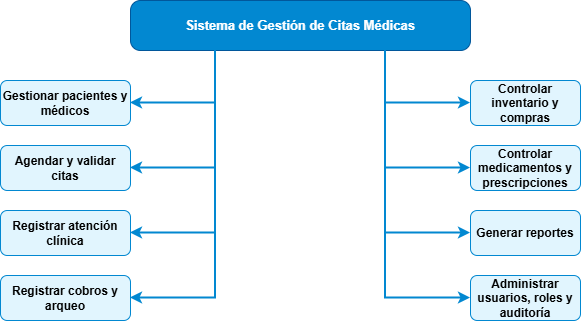
\includegraphics[width=\textwidth,height=0.52\textheight,keepaspectratio]{diagramas/draw1.png}
\caption{Funciones principales del sistema.}
\label{fig:funciones-principales}
\end{figure}

\section{Conversión de funciones en componentes}

Las funciones se agrupan en componentes cohesivos para separar responsabilidades y facilitar el mantenimiento del sistema. La agenda concentra las operaciones de citas; el componente clínico administra la atención y los consumos; y los componentes financiero, de inventario y de seguridad gestionan sus respectivos dominios.

\begin{figure}[htbp]
\centering
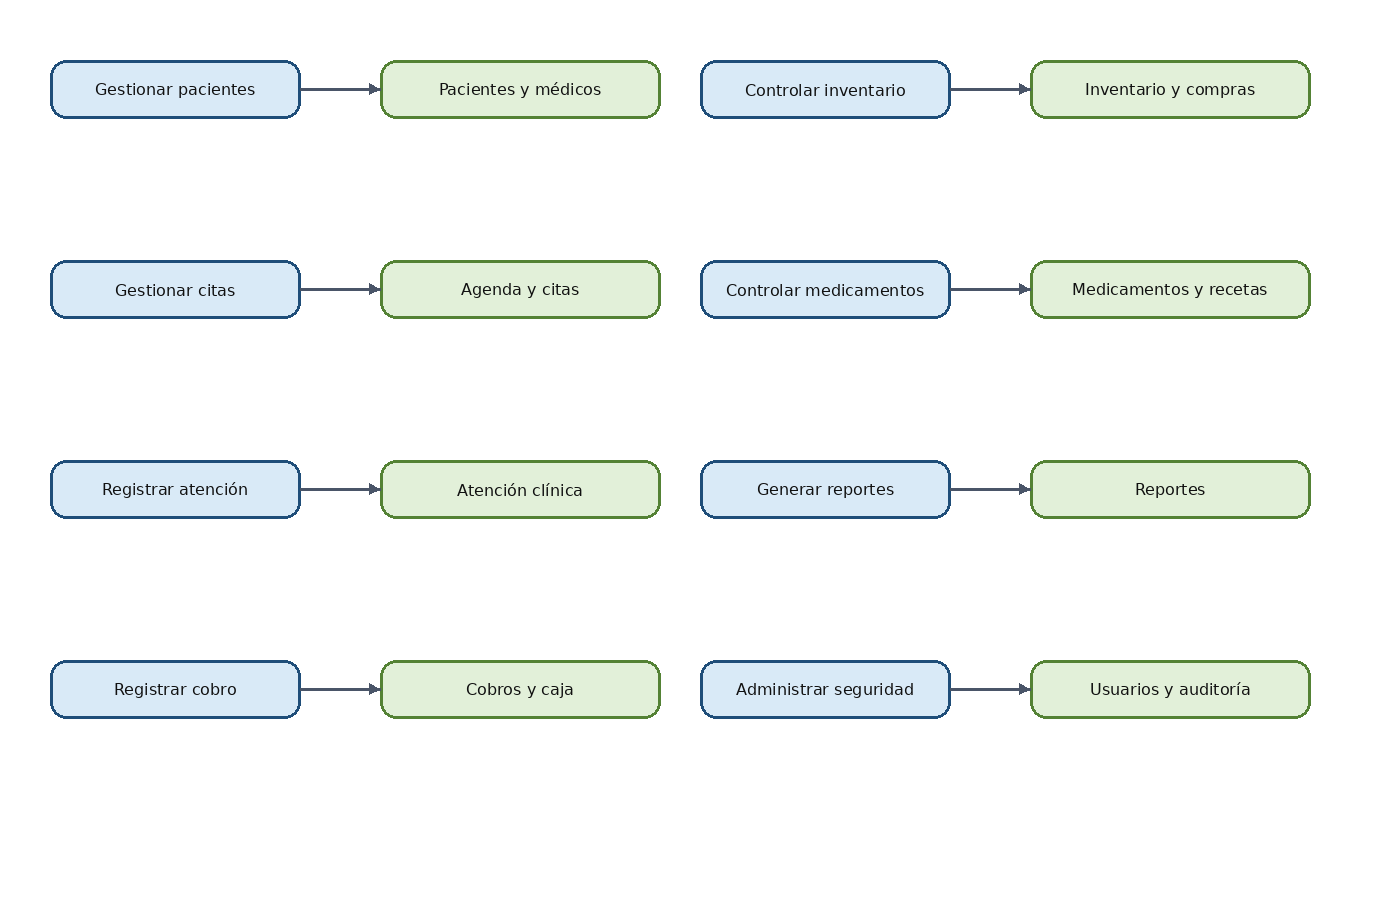
\includegraphics[width=\textwidth,height=0.52\textheight,keepaspectratio]{diagramas/draw2.png}
\caption{Correspondencia entre funciones y componentes del sistema.}
\label{fig:funciones-componentes}
\end{figure}

\section{Responsabilidades de los componentes}

La siguiente tabla establece qué información y operaciones administra cada componente identificado.

\small
\begin{tabularx}{\textwidth}{>{\bfseries}p{0.30\textwidth}X}
\toprule
\rowcolor{azulprincipal}\textcolor{white}{Componente} & \textcolor{white}{¿De qué se encarga?}\\
\midrule
Gestión de pacientes y médicos & Registrar y actualizar pacientes, médicos, especialidades, horarios y datos básicos necesarios para la atención.\\
Agenda y citas & Crear, consultar, modificar y cancelar citas; validar disponibilidad; controlar estados e historial de cambios.\\
Atención clínica & Registrar la atención, notas clínicas permitidas, prescripciones y consumos de insumos durante procedimientos.\\
Cobros y caja & Registrar montos, medios y estados de pago; generar el arqueo diario y bloquear modificaciones posteriores al cierre.\\
Inventario y compras & Administrar insumos, existencias, stock mínimo, entradas, salidas, consumos, proveedores y facturas.\\
Medicamentos y prescripciones & Vincular medicamentos sujetos a receta con el paciente, la consulta y la prescripción válida.\\
Reportes & Generar reportes de citas, cobros, compras, productividad médica e inventario con filtros por fecha.\\
Usuarios, roles y auditoría & Autenticar usuarios, autorizar operaciones según el rol y registrar usuario, fecha, hora y motivo de los cambios.\\
\bottomrule
\end{tabularx}
\normalsize

\begin{figure}[htbp]
\centering
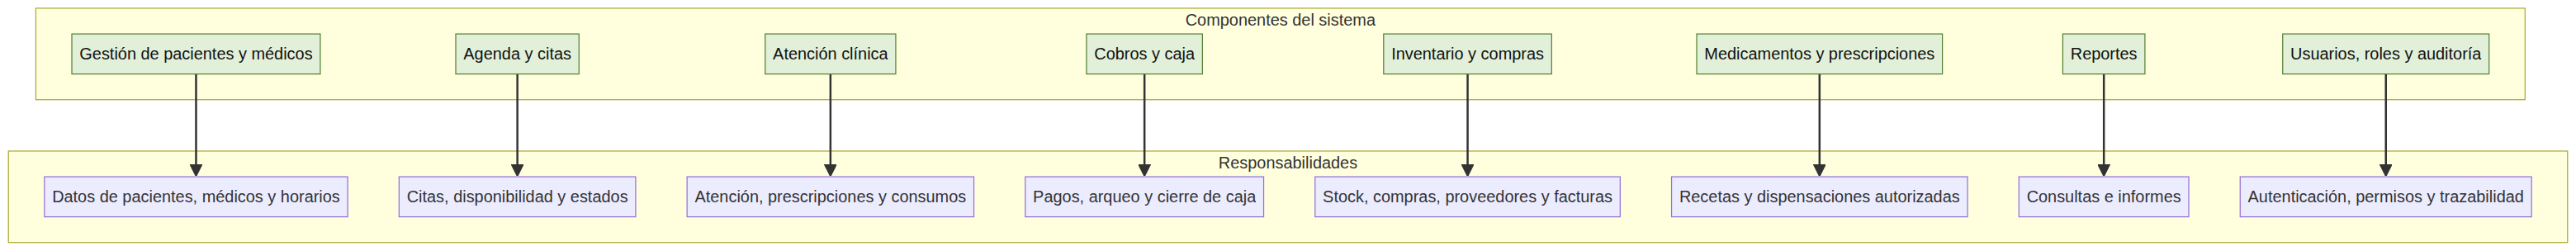
\includegraphics[width=\textwidth,height=0.52\textheight,keepaspectratio]{diagramas/draw3.png}
\caption{Componentes y responsabilidades principales.}
\label{fig:responsabilidades}
\end{figure}

\section{Relaciones entre componentes}

Las relaciones se definen mediante dependencias funcionales. La agenda utiliza pacientes y médicos para crear citas; la atención clínica consulta la agenda y descuenta los consumos del inventario; los cobros se relacionan con las citas; y los reportes consultan la información consolidada sin modificarla.

\begin{figure}[htbp]
\centering
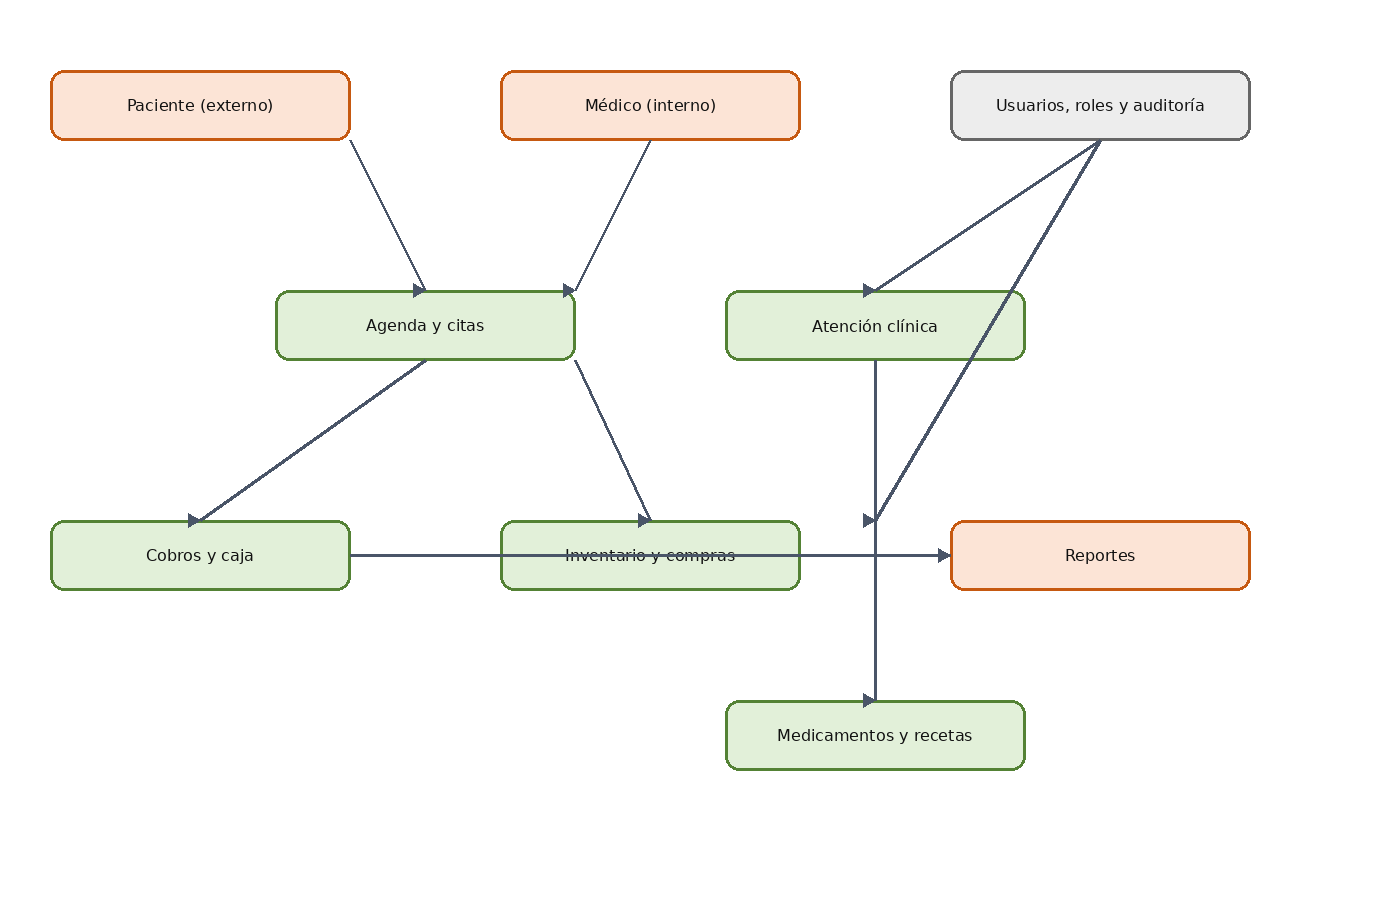
\includegraphics[width=\textwidth,height=0.52\textheight,keepaspectratio]{diagramas/draw4.png}
\caption{Relaciones y dependencias entre componentes.}
\label{fig:relaciones}
\end{figure}

\section{Usuarios del sistema}

Los usuarios y actores definidos en la captura de requerimientos interactúan con diferentes componentes según sus responsabilidades:

\begin{itemize}
    \item \textbf{Recepcionista:} registra pacientes, agenda citas, consulta disponibilidad, registra cobros y realiza el arqueo autorizado.
    \item \textbf{Médico:} consulta su agenda, registra la atención, emite prescripciones y declara los insumos consumidos.
    \item \textbf{Administrador:} administra usuarios, médicos, inventario, compras, parámetros y reportes.
    \item \textbf{Gerente general:} consulta información consolidada y reportes para supervisar la clínica.
    \item \textbf{Paciente:} proporciona sus datos, solicita citas y recibe confirmaciones o avisos.
\end{itemize}

\begin{figure}[htbp]
\centering
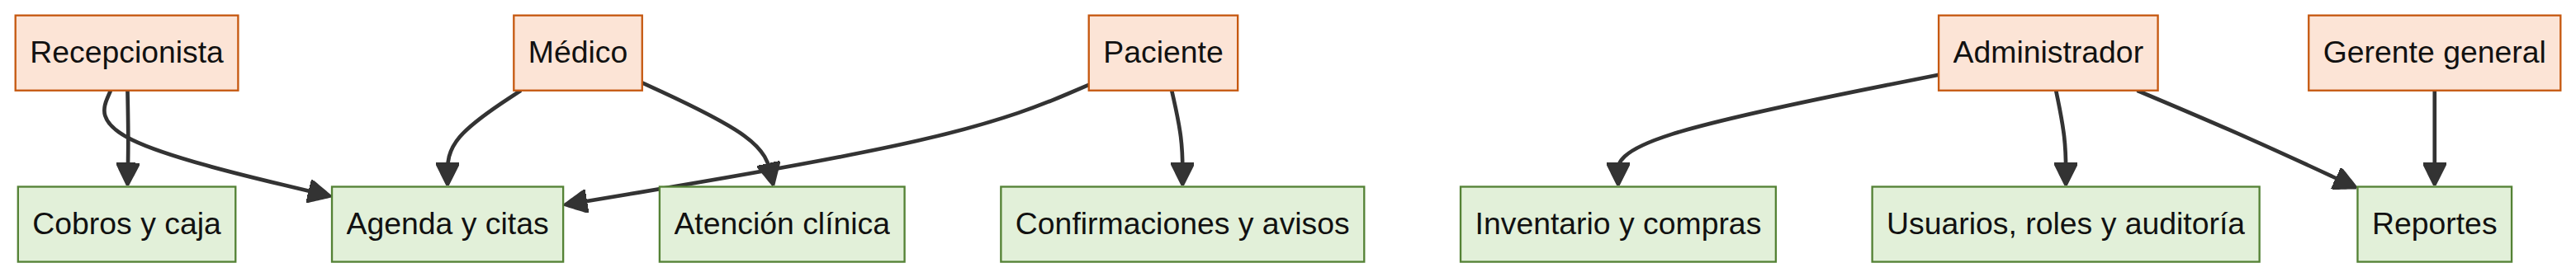
\includegraphics[width=\textwidth,height=0.52\textheight,keepaspectratio]{diagramas/draw5.png}
\caption{Usuarios y componentes con los que interactúan.}
\label{fig:usuarios}
\end{figure}

\section{Base de datos del sistema}

La base de datos debe centralizar la información y conservar la trazabilidad. Como mínimo, se identifican las entidades Paciente, Médico, Usuario, Cita, Atención, Prescripción, Medicamento, Insumo, Movimiento de inventario, Proveedor, Compra, Cobro y Auditoría. Las relaciones deben impedir citas solapadas, controlar existencias no negativas y vincular cobros y prescripciones con la atención correspondiente.

\begin{figure}[htbp]
\centering
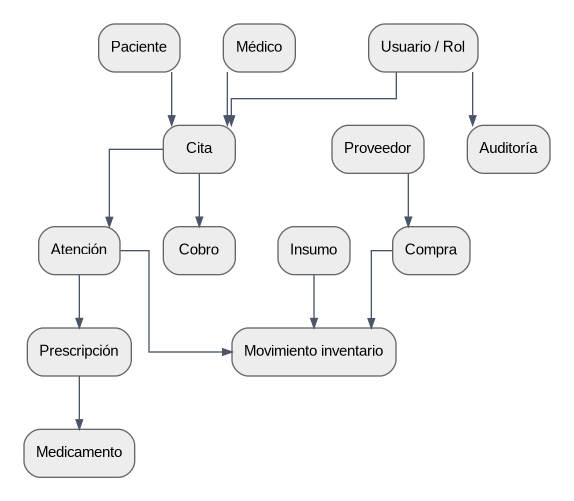
\includegraphics[width=\textwidth,height=0.52\textheight,keepaspectratio]{diagramas/draw6.png}
\caption{Base de datos conceptual y sus relaciones principales.}
\label{fig:base-datos}
\end{figure}

\section{Arquitectura del sistema}

Se propone una arquitectura por capas. La capa de presentación atiende las operaciones de los usuarios; la capa de aplicación coordina los casos de uso y aplica las reglas de negocio; la capa de dominio concentra las entidades y validaciones; y la capa de datos persiste la información. Los servicios transversales de autenticación, auditoría, reportes y respaldo apoyan a todas las capas.

Esta separación permite modificar la interfaz sin alterar las reglas de negocio, facilita las pruebas y protege la información clínica y administrativa mediante controles de acceso.

\begin{figure}[htbp]
\centering
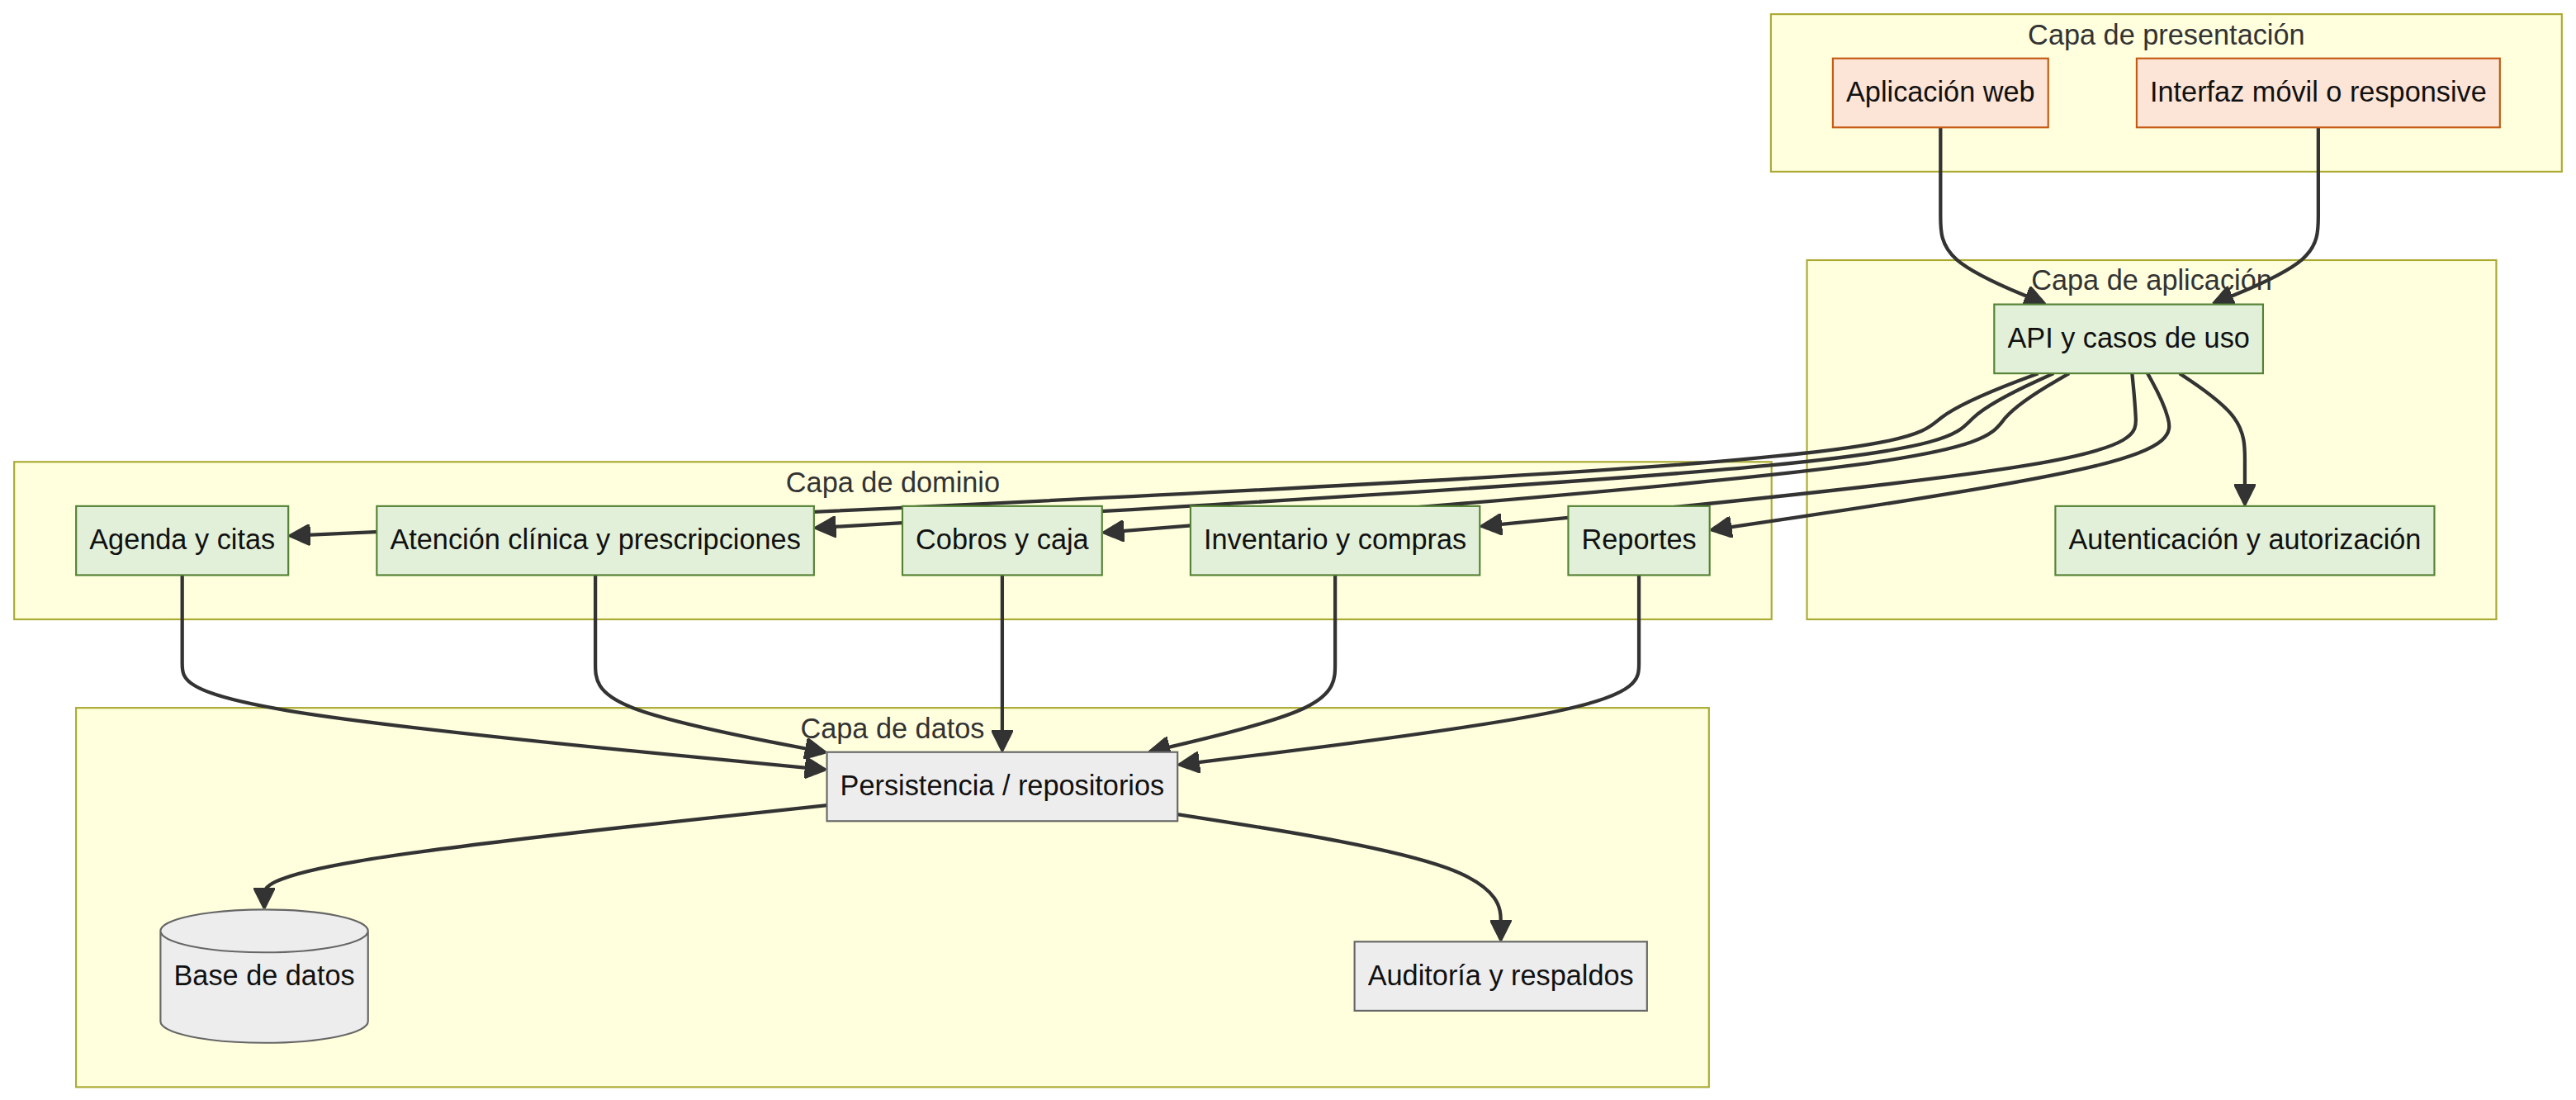
\includegraphics[width=\textwidth,height=0.52\textheight,keepaspectratio]{diagramas/draw7.png}
\caption{Arquitectura propuesta del sistema de gestión de citas médicas.}
\label{fig:arquitectura}
\end{figure}

\subsection*{Conclusión de la propuesta}

La solución transforma el proceso manual identificado en la entrevista en una arquitectura modular y trazable. Los componentes propuestos cubren las funciones prioritarias del proyecto, incorporan explícitamente a los usuarios y a la base de datos, y permiten implementar gradualmente la agenda, la atención clínica, los cobros, el inventario y los reportes.

\clearpage
\setcounter{section}{0}
\section*{MODELADO BPMN Y UML DEL SISTEMA DE GESTIÓN DE CITAS MÉDICAS}
\begin{center}
\textit{Adaptación de los ejemplos de clase al proceso de agendamiento y atención de citas}
\end{center}

\section{Criterio de adaptación}

Los materiales de referencia presentan un proceso de inventario y recepción de productos. Para este proyecto se conserva la metodología enseñada: identificar participantes, actividades, decisiones, eventos, flujos de mensaje y responsabilidades. El contenido se adapta al dominio médico, en el que participan el paciente, la clínica, recepción, el médico y caja o administración.

El proceso seleccionado para modelar es \textbf{Agendar y atender una cita médica}, porque conecta los requerimientos prioritarios del proyecto: disponibilidad del médico, registro de la cita, atención clínica, cobro y actualización de la información.

\section{Caso de uso: Gestionar cita médica}

\begin{tabularx}{\textwidth}{>{\bfseries}p{0.28\textwidth}X}
\toprule
\rowcolor{azulprincipal}\textcolor{white}{Elemento} & \textcolor{white}{Descripción}\\
\midrule
Actor principal & Recepcionista\\
Actores secundarios & Paciente, Médico y Administrador\\
Caso de uso & Gestionar cita médica\\
Objetivo & Registrar una cita sin solapamientos, confirmar la atención, registrar el resultado de la consulta y asociar el cobro correspondiente.\\
Precondiciones & El usuario debe estar autenticado; el paciente y el médico deben estar registrados; debe existir un horario disponible.\\
Resultado exitoso & La cita queda registrada y atendida o confirmada, el cobro queda asociado y la información clínica permitida se conserva.\\
Flujo alternativo & Si no existe disponibilidad, el sistema informa el conflicto y permite seleccionar otro horario.\\
\bottomrule
\end{tabularx}

\begin{figure}[htbp]
\centering
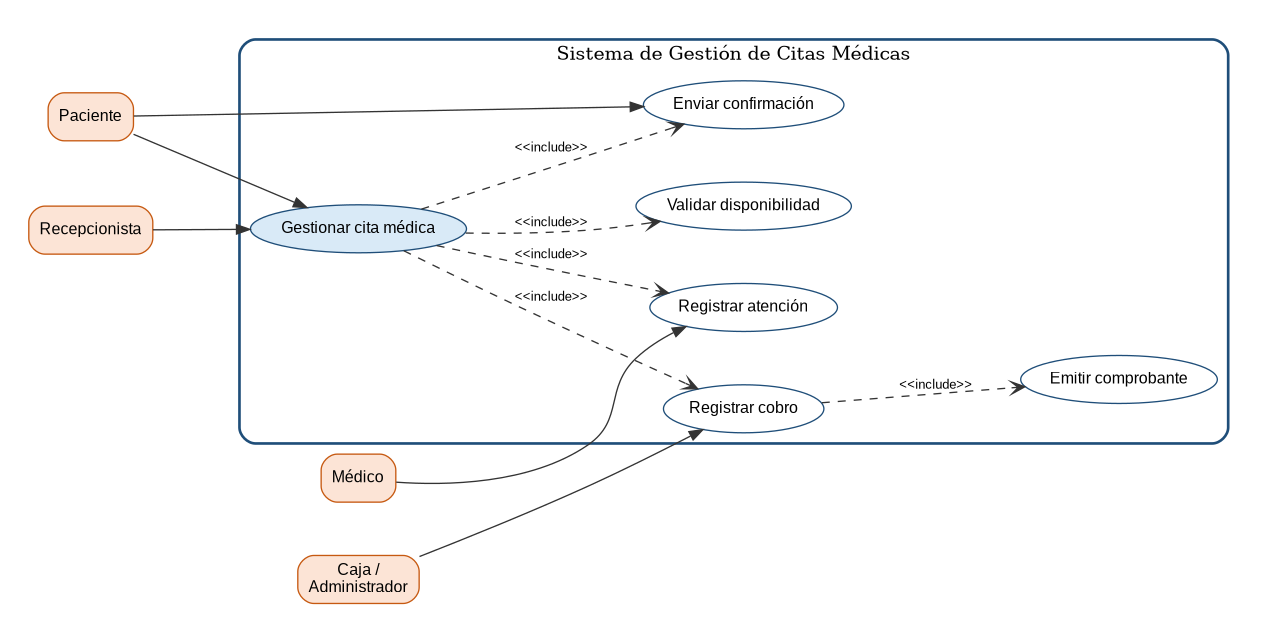
\includegraphics[width=\textwidth,height=0.50\textheight,keepaspectratio]{modelado/caso_uso_citas.png}
\caption{Caso de uso y actores de Gestionar cita médica.}
\label{fig:caso-uso-citas}
\end{figure}

\section{BPMN 2.0: Agendar y atender cita}

\subsection*{Participantes y lanes}

\begin{itemize}
    \item \textbf{Pool 1: Paciente:} solicita la cita y recibe la confirmación o el aviso de indisponibilidad.
    \item \textbf{Pool 2: Clínica:} contiene los lanes Recepción, Médico y Caja/Administración.
    \item \textbf{Lane Recepción:} registra al paciente, consulta disponibilidad y agenda la cita.
    \item \textbf{Lane Médico:} atiende la cita, registra la atención y emite una prescripción cuando corresponde.
    \item \textbf{Lane Caja/Administración:} registra el cobro, emite el comprobante y consulta reportes.
\end{itemize}

\subsection*{Flujo del proceso}

El proceso comienza cuando el paciente solicita una cita. Recepción consulta la disponibilidad del médico. La compuerta exclusiva determina si existe un horario libre: si no existe, se informa al paciente y termina el flujo alternativo; si existe, se registra y confirma la cita. En la fecha programada, el médico atiende al paciente y registra la atención. Finalmente, caja registra el cobro y genera el comprobante.

\begin{figure}[htbp]
\centering
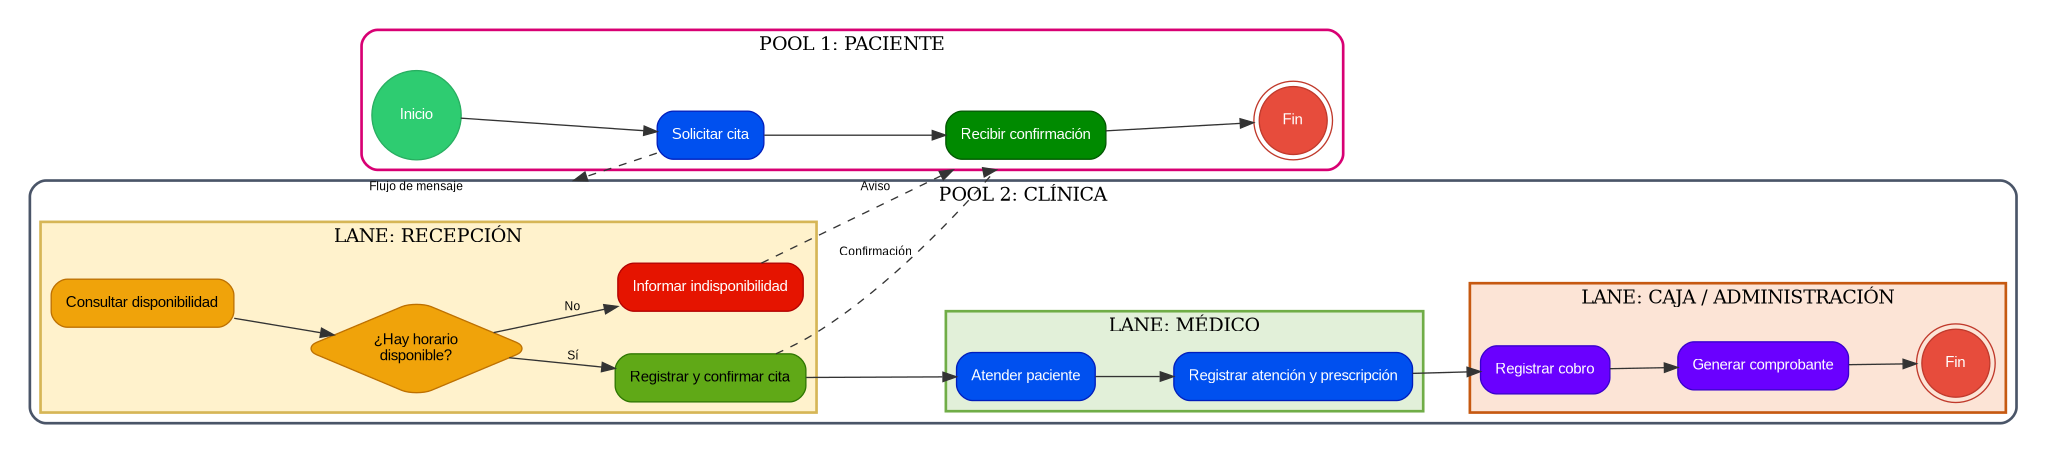
\includegraphics[width=\textwidth,height=0.50\textheight,keepaspectratio]{modelado/bpmn_citas.png}
\caption{Modelo BPMN del proceso de agendamiento y atención.}
\label{fig:bpmn-citas}
\end{figure}

\section{Diagrama de actividades UML}

El diagrama de actividades representa el flujo interno del sistema con dos responsables: Recepción y Sistema. La decisión principal es ``¿Existe disponibilidad?''. El ciclo ``¿Registrar otra cita?'' representa que el usuario puede continuar gestionando citas sin cerrar la sesión.

\begin{figure}[htbp]
\centering
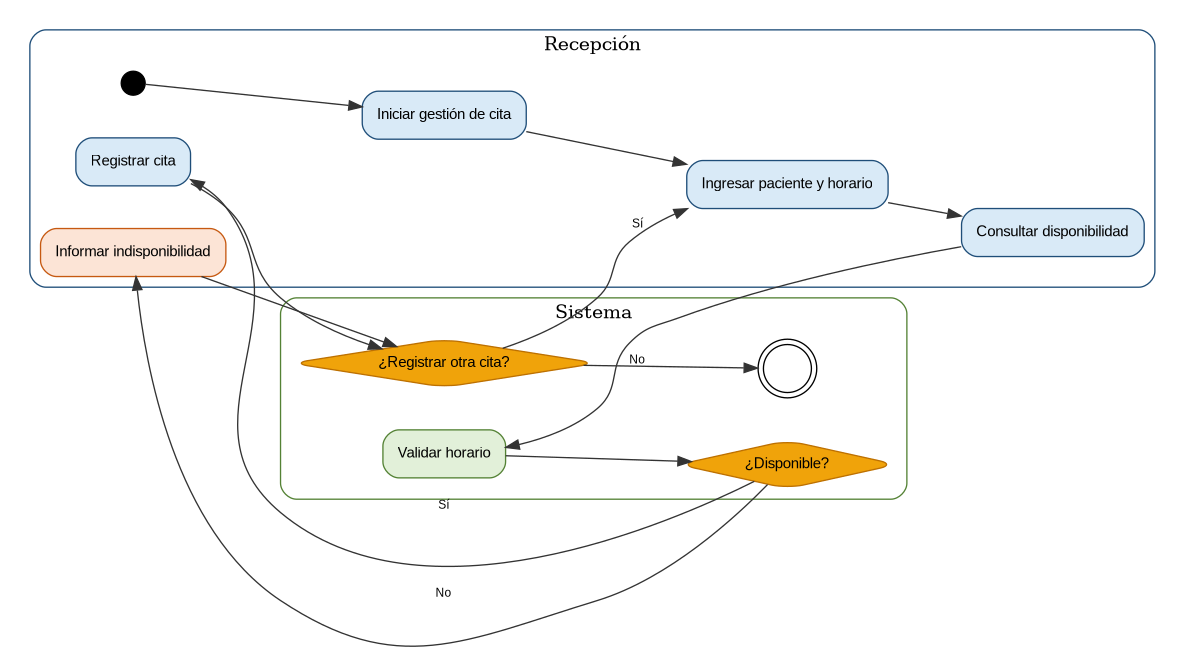
\includegraphics[width=\textwidth,height=0.50\textheight,keepaspectratio]{modelado/actividad_citas.png}
\caption{Diagrama de actividades UML para gestionar una cita.}
\label{fig:actividad-citas}
\end{figure}

\section{Diagrama de secuencia UML}

Los participantes de la interacción son Paciente, Interfaz de Citas, Gestor de Agenda, Médico, Servicio de Cobro y Base de Datos. La condición \texttt{[disponible]} permite guardar la cita; la condición \texttt{[no disponible]} devuelve un mensaje al paciente. La estructura \texttt{loop} representa la consulta o registro de varias citas durante la jornada.

\begin{figure}[htbp]
\centering
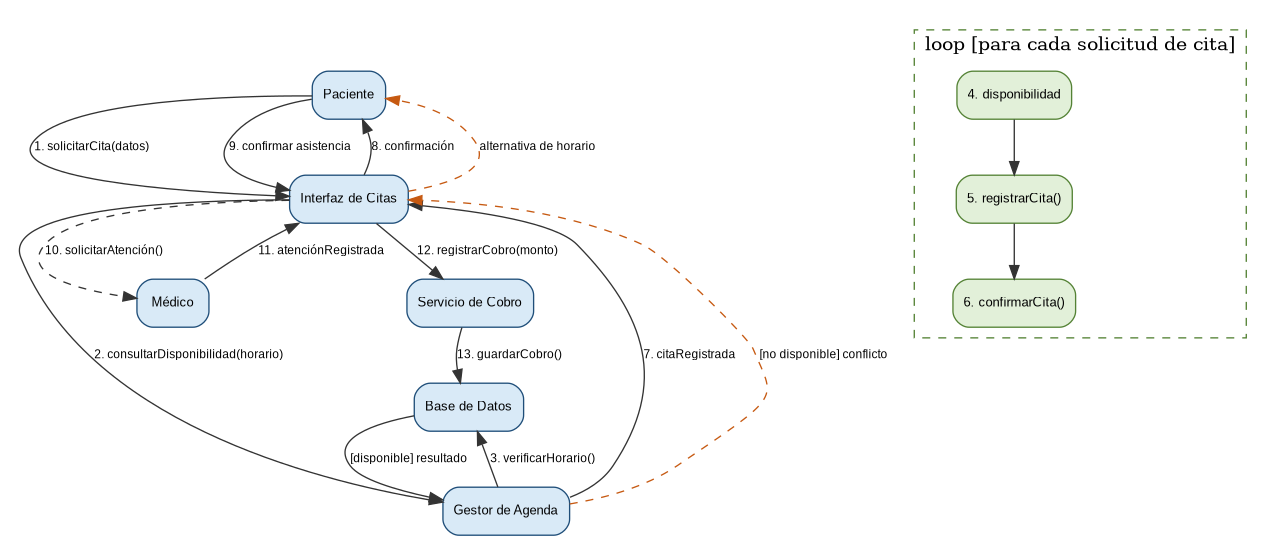
\includegraphics[width=\textwidth,height=0.50\textheight,keepaspectratio]{modelado/secuencia_citas.png}
\caption{Diagrama de secuencia UML para gestionar una cita.}
\label{fig:secuencia-citas}
\end{figure}

\section{Trazabilidad con los requerimientos}

\begin{tabularx}{\textwidth}{>{\bfseries}p{0.22\textwidth}p{0.30\textwidth}X}
\toprule
\rowcolor{azulprincipal}\textcolor{white}{Modelo} & \textcolor{white}{Requerimientos relacionados} & \textcolor{white}{Evidencia en el modelo}\\
\midrule
Caso de uso & RF-001, RF-002, RF-003 & El actor inicia la gestión, se valida la disponibilidad y se registra el cobro.\\
BPMN & RF-001, RF-002, RN-01 & Pools, lanes, flujo de mensajes y compuerta exclusiva para evitar citas solapadas.\\
Actividades UML & RF-001, RF-002 & Secuencia de tareas, decisión de disponibilidad y repetición del proceso.\\
Secuencia UML & RF-001, RF-002, RF-003, RNF-001 & Mensajes entre interfaz, gestor, médico, cobro y base de datos.\\
\bottomrule
\end{tabularx}

\subsection*{Observación técnica}

El BPMN describe la colaboración entre participantes del proceso de negocio; los diagramas UML detallan el comportamiento funcional del software. Por ello, ambos modelos se complementan y no deben sustituirse entre sí.


\end{document}
